\documentclass[a4paper]{article}

%%%%%%%% CREATE DOCUMENT STRUCTURE %%%%%%%%
%% Language and font encodings
\usepackage[english]{babel}
\usepackage[utf8x]{inputenc}
\usepackage[T1]{fontenc}
\usepackage{multirow}
\usepackage{dingbat}
\usepackage{tabulary,booktabs}
\usepackage{listings}
\usepackage{xparse}


\usepackage{amsmath,amssymb,amsthm}
\usepackage[table,xcdraw]{xcolor}
\usepackage[center]{caption}
\usepackage{scrextend}
\usepackage{comment}
%\usepackage{subfig}

%% Sets page size and margins
\usepackage[a4paper,top=3cm,bottom=2cm,left=2cm,right=2cm,marginparwidth=1.75cm]{geometry}

%% Useful packages
\usepackage{amsmath}
\usepackage{graphicx}
\usepackage[colorinlistoftodos]{todonotes}
\usepackage[colorlinks=true, allcolors=blue]{hyperref}
\usepackage{caption}
\usepackage{subcaption}
\usepackage{sectsty}
\usepackage{apacite}
\usepackage{float}
\usepackage{titling} 
\usepackage{blindtext}
\usepackage[square,sort,comma,numbers]{natbib}
\usepackage[colorinlistoftodos]{todonotes}
\usepackage{xcolor}
\definecolor{darkgreen}{rgb}{0.0, 0.4, 0.0}

\usepackage{courier}

\lstset{basicstyle=\footnotesize\ttfamily,breaklines=true}
\lstset{framextopmargin=50pt,frame=bottomline}

%%%%%%%% DOCUMENT %%%%%%%%
\begin{document}

%%%% Title Page
\begin{titlepage}

\newcommand{\HRule}{\rule{\linewidth}{0.5mm}} 							% horizontal line and its thickness
\center 
 
% University
\textsc{\LARGE Eindhoven University of Technology}\\[1cm]

% Document info
\textsc{\Large Embedded Computer Architecture } \\[0.2cm]
\textsc{\large 5SIA0 }\\[1cm] 										% Course Code
\HRule \\[0.8cm]
{ \huge \bfseries EEG Application Feature Optimization by Porting C Algorithms to CUDA for Nvidia GPU Utilization }\\[0.6cm]								% Assignment
\HRule \\[2cm]
\large
\emph{Authors:}\\
Christopher Ohara (1322884) \\
Erik Wouters (1325892) \\	
[1.5cm]	
% Author info
{\large \today}\\[5cm]

\includegraphics[width=0.6\textwidth]{images/TUE-Logo.jpg}\\[1cm] 	% University logo
\vfill 
\end{titlepage}


%%%% SECTIONS

\section{Introduction}

This assignment requires us to port an application to process \texttt{EEG signals} to run on a GPU. This provides insight in how to achieve the shortest run time for a given application and GPU. The following sections discuss the techniques used in this assignment.

\subsection{The EEG Application}

The \texttt{EEG} application used in this assignment uses six different algorithms to compare a dataset of \texttt{EEG} signals. The structure of the application is depicted in Figure \ref{fig:eeg}. The algorithms used are:
\begin{itemize}
\item Butterworth Filter (\texttt{BF})
\item Standard Features (\texttt{StdF})
\item Peak to Peak Features (\texttt{P2P})
\item Approximate Entropy Feature (\texttt{ApEn})
\item Hurst Coefficient Feature (\texttt{H})
\item Power Spectral Density Feature (\texttt{PSD})
\end{itemize}

\begin{figure}[H]
\begin{center}
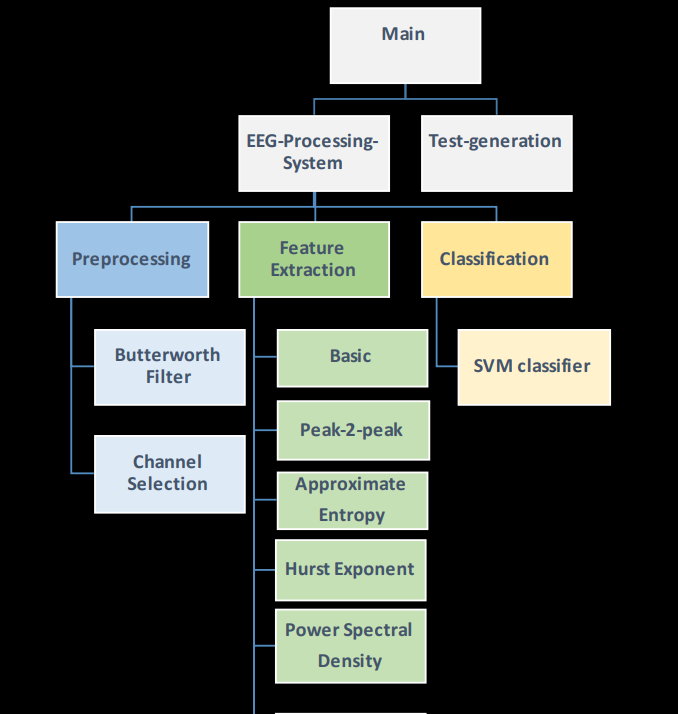
\includegraphics[scale=0.3]{images/EEG_Overview.PNG}
\caption{Overview of the structure of the EEG application, as given in ECA.}
\label{fig:eeg}
\end{center}
\end{figure}


\subsection{Execution Time} 
It is crucial to find out which part of the application consumes the most time. The average execution time (over the \texttt{23 channels}) of each of the six features when run on the CPU can be found in Table \ref{tab:CPU}. For example, the \texttt{Approximate Entropy Feature} (\texttt{ApEn}) takes at least two orders of magnitude more time to execute than the other features. If we can make this function \texttt{2x} \textit{faster}, the program will also be about \texttt{2x} \textit{faster}. If to the contrary we would make each of the other features run \texttt{10x} \textit{faster} the speedup would be \texttt{zero} because they represent such a small portion of the total execution time.
\\

\noindent To time the program, the \texttt{time.h} library has been included. The following defines have been added to the header file \texttt{eeg.h}. If \texttt{TIMING} is defined, the total execution time will be printed. If \texttt{TIMING\_ALL} is defined the execution time of each of each feature and channel will be printed. Finally, if \texttt{TIMING\_CSV} is defined, the times will be printed in a nice, comma-separated value format. The following code was added to the calls to each of the features:
\begin{lstlisting}
#ifdef TIMING_ALL
	clock_t begin = clock();
#endif

//... Call to feature

#ifdef TIMING_ALL
	clock_t end = clock();
	double time = (double)(end - begin) / CLOCKS_PER_SEC;
	#ifdef TIMING_CSV
		printf("%lf,", time);
	#else
		printf("Time: %lfs\r\n", time);
	#endif
#endif
\end{lstlisting}

\begin{table}[h!]
\begin{center}  
\begin{tabular}{| l | c |}
\hline
\rowcolor[HTML]{c0c0c0}
\multicolumn{1}{| c |}{Feature} & Execution Time [s]\\ \hline
Butterworth Filter & 0.000429\\ \hline
Standard Features & 0.000528\\ \hline
Peak to Peak Features & 0.000275\\ \hline
Approximate Entropy Feature & 4.262079\\ \hline
Hurst Coefficient Feature & 0.001439\\ \hline
Power Spectral Density Feature & 0.019520\\ \hline
\end{tabular}
\caption{Execution time of EEG application on the CPU using the \texttt{g++} compiler.}
\label{tab:CPU}
\end{center}
\end{table}

\subsection{Dataset}
The dataset consists of \texttt{23 channels} with \texttt{256 samples} each. Of course, problems large enough to need a GPU performance boost amortize the overhead better than small problems. It is worth noting that in a real world \texttt{EEG application}, the dataset would contain many more samples, which should amplify the effects of any speedup in the application. 

\subsection{Test System}

Included in the appendix are the test system specifications. These specifications are important to report in order to recreate the experiment with similar results (as even server utilization can impact results). The key parameters are the \texttt{Compute Capability}, \textit{maximum} \texttt{Grid} and \texttt{Block Dimensions} and \texttt{Threads per Warp}. While relatively small dimensions are used (for this exercise), the maximum value allows for larger datasets, given by \texttt{BLOCK\_SIZE*GRID\_SIZE}. The server used for experimentation is a dedicated TU/e server with three GeForce GTX 570 GPUs which lives at $co13.ics.ele.tue.nl$. The connection to this server was made over \texttt{ssh}, \texttt{sftp}, \texttt{git} and \texttt{X Server} using \texttt{MobaXterm}.

\section{CUDA}
Because the test system has an \texttt{NVIDIA} GPU, we will use the \texttt{CUDA Toolkit}. The toolkit comes with many libraries of algorithms that are implemented to run in parallel on the GPU. For example the \texttt{cufft.h} library that will be used for the Fast Fourier Transform that is used in the Power Spectral Density feature. It also includes functions to manage the GPU memory and the \texttt{CUDA cores} that run the algorithms in parallel.

\noindent When a \texttt{CUDA} function is called the GPU will take some time to warm-up. This takes approximately 0.6 seconds. In order to \textit{avoid} the effects of this, a \texttt{dummy} call is added to the GPU at the beginning of the main function.

\begin{lstlisting}
    #ifndef CPU_ONLY
    // dummy function
    int32_t* dummy;
    cudaMallocManaged(&dummy, sizeof(int32_t));
    cudaFree(dummy);
    #endif
\end{lstlisting}

\noindent Directly converting \texttt{.c} files to \texttt{.cu} files and compiling them with \texttt{nvcc} makes them execute in approximately \texttt{3x} \textit{more} time than \texttt{.c} compiled with \texttt{g++}. This must be taken into account when porting applications to the GPU. If there is a lot of code in a file that will not be run on the GPU, the file should be split in a part that contains the CPU code and is compiled with for instance \texttt{g++}, and a file with almost exclusively code that will run on the GPU and is compiled with \texttt{nvcc}.
\\

\noindent To use the \texttt{CUDA} profiling tools the two commands below were added to the \texttt{Makefile}. The command "\texttt{make profile}" runs the compiled code and collects the time spent in each of the \texttt{CUDA} library functions. This is very useful to see which functions take the most time on average. An example of the output of this command for the final executable is included in the appendix.
The command "\texttt{make nvvp}" starts the \texttt{NVIDIA Visual Profiler} (\texttt{NVVP}), which has been used to create the figures with the detailed time-lines of the execution of the EEG application.
\begin{lstlisting}
profile:$(EXE)
	nvprof --system-profiling on ./$(EXE)
nvvp:$(EXE)
	nvvp ./$(EXE)
\end{lstlisting}

\section{Strategy}
Based on \texttt{Amdahl's Law}, it is known that the primary task should be to optimize functions (features) that are the \textit{most} resource intensive. Analyzing the results in Table \ref{tab:CPU} shows that the Approximate Entropy (\texttt{ApEn}) and Power Spectral Density (\texttt{PSD}) features have the highest impact on the execution time. For the \texttt{ApEn} feature, the loop requirements were optimized. For the \texttt{PSD} feature, a \texttt{CUDA} version of the Fast Fourier Transform (\texttt{cuFFT}) will be explored in this report.

\section{Optimization}

\subsection{Standard Features}

In order to gain familiarity with porting \texttt{C} algorithms to \texttt{CUDA}, it is important to determine a feasible application with the least amount of effort. First the \texttt{gpu\_average()} has been ported to the GPU to gain familiarity with the process. The time-line of the execution of this function on the GPU can be found in Figure \ref{fig:GPU_avg}. The actual execution for a single channel is very short, so a zoomed in version of the execution of the \texttt{kernel} has been provided in Figure \ref{fig:GPU_avg_detail}.

As a result of porting this standard feature, running the \texttt{abssum} on the GPU with \texttt{CUDA} caused the standard features set to run \texttt{3x} \textit{slower} than the \texttt{CPU\_ONLY}. This result seems reasonable based on what was previously discussed in the \texttt{CUDA} section above. Considerations were given to remove this feature "optimization" but since the goal is to have a functioning implementation that scales with data points, it was kept in. Therefore, data representation could have been reported with a higher overall speedup at the cost of making this program a one-time-use for this specific dataset. 

\begin{figure}[H]
\begin{center}
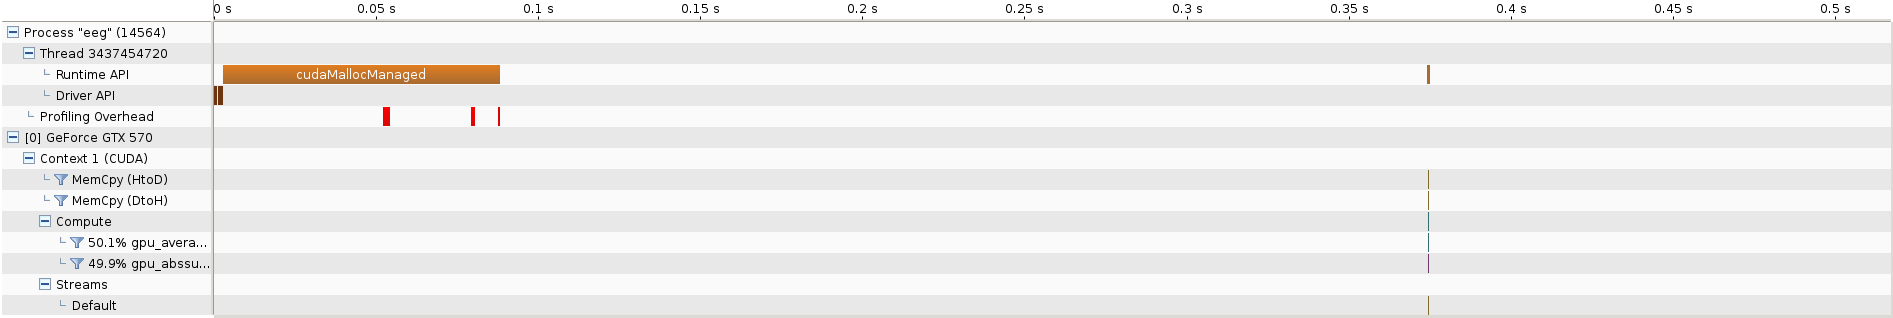
\includegraphics[scale=0.35]{images/07_cuda_startup.PNG}
\caption{Execution time-line of the port of the \texttt{gpu\_average()} in NVVP.}
\label{fig:GPU_avg}
\end{center}
\end{figure}

\begin{figure}[H]
\begin{center}
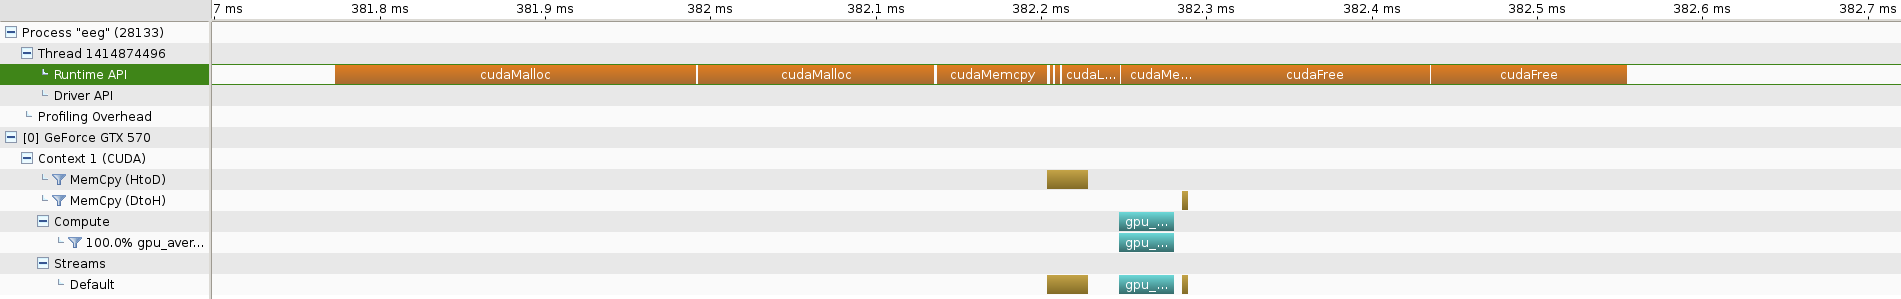
\includegraphics[scale=0.35]{images/06_detail_cudaMallocManaged.PNG}
\caption{Detailed time-line of the execution of \texttt{gpu\_average()} for a single channel in NVVP. By far the most time is spent in the memory management functions.}
\label{fig:GPU_avg_detail}
\end{center}
\end{figure}

To illustrate that the GPU speed-up becomes more interesting when intertwining algorithms the \texttt{gpu\_abssum()} has also been ported to the GPU. Because this algorithm uses the exact same data as the \texttt{gpu\_average()}, it is runs very quickly and does not require to copy the data to the GPU again. The result of this execution can be seen in Figure \ref{fig:GPU_abs_detail}.

\begin{figure}[H]
\begin{center}
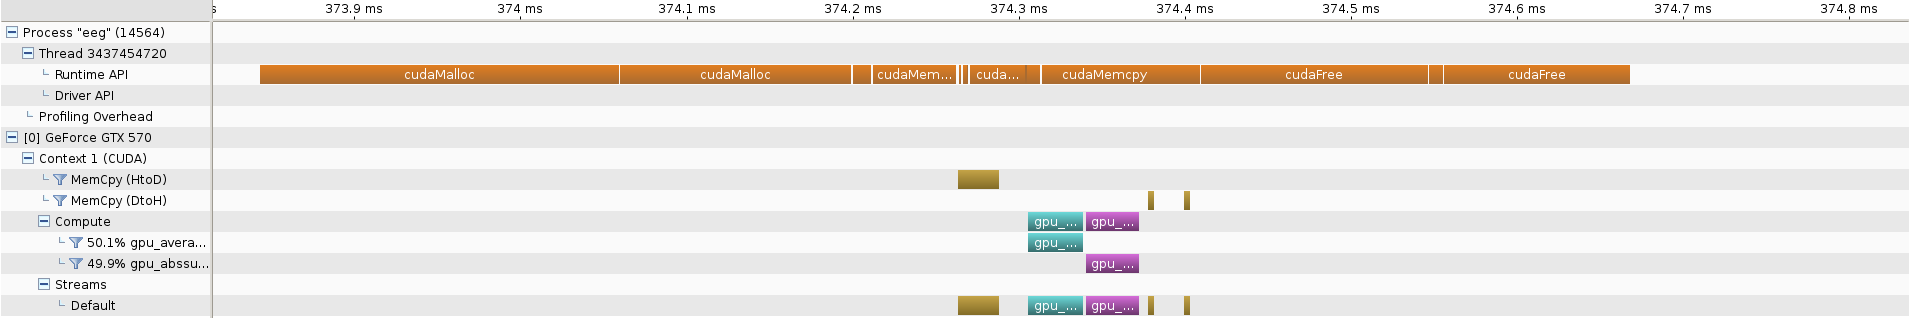
\includegraphics[scale=0.35]{images/06_detail_cudaMallocManaged_with_sta.PNG}
\caption{Detailed time-line of the execution of \texttt{gpu\_average()} and \texttt{gpu\_abssum()} for a single channel in NVVP. The execution of the algorithms is intertwined, reducing the overhead for allocating memory on the GPU. The more features that can be ported to run on the same data, the more the overhead of using the GPU can be reduced, since the \texttt{cudaFree} and \texttt{cudaMallocManaged} functions take up the majority of the time.}
\label{fig:GPU_abs_detail}
\end{center}
\end{figure}


\subsection{Approximate Entropy Feature}

The \texttt{ApEn} feature is optimized via halving the number of iterations by only iterating over the lower triangle of $i$ and $j$ and exiting also when $i==j$. This allows the program to minimize redundant calculations in the \texttt{apen\_correlation} algorithm, since the resulting matrix is symmetric over the diagonal. However, \texttt{CUDA} needs the loop exit condition $i>j$, since it maps a 2D block into a 1D vector and then stores the \texttt{counts} into \texttt{blocksums}.

\begin{figure}[H]
\begin{center}
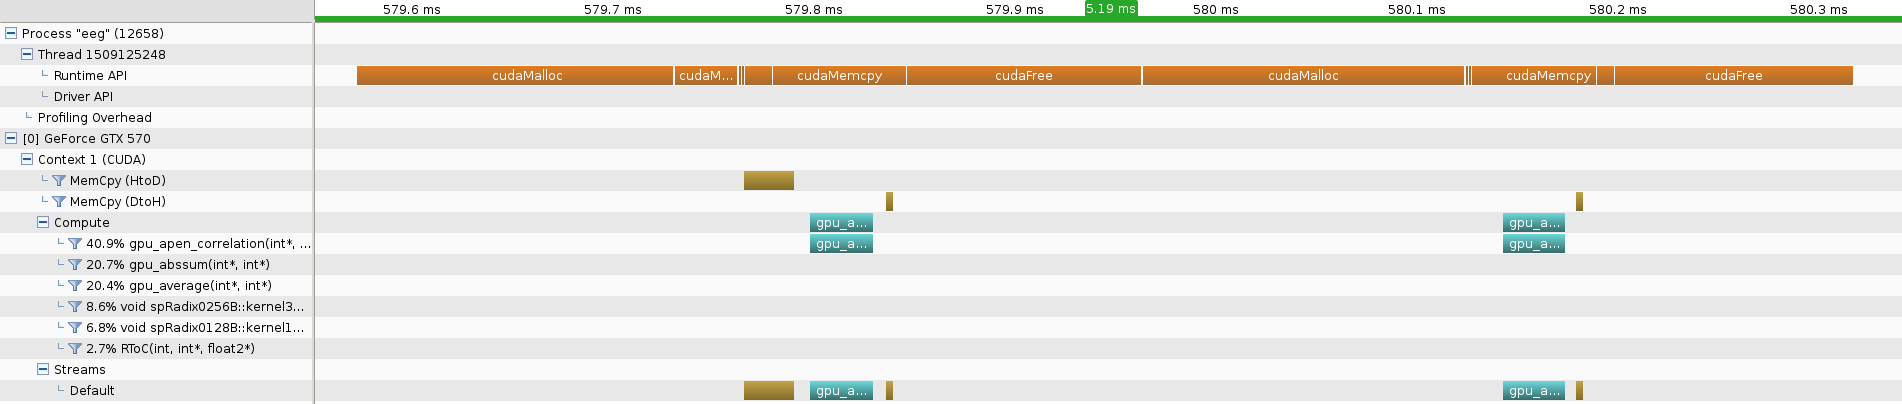
\includegraphics[scale=0.35]{images/09_cuda_apen_detail.PNG}
\caption{Detailed time-line of the execution of \texttt{apen\_correlation()} for a single channel in NVVP. By far the most time is spent in the memory management functions.}
\label{fig:GPU_apen_detail}
\end{center}
\end{figure}

\noindent Reference: GPU code for \texttt{ApEn}.
\begin{lstlisting}
__global__
void gpu_apen_correlation(int32_t *device_x, double *blocksums, int np, unsigned int m, double r)
{
	unsigned int i = blockIdx.y*blockDim.y+threadIdx.y;
	unsigned int j = blockIdx.x*blockDim.x+threadIdx.x;
	bool set=false;
	unsigned int index = threadIdx.y*BLOCK_SIZE+threadIdx.x;
	__shared__ int32_t counts[1024];   
	__syncthreads();
	if (i==j && i <= np - (m + 1) + 1 && j <= np - (m + 1) + 1)
		counts[index] = 1;
	else if (j < i)
		counts[index] = 0;
	else {
		for (unsigned int k = 0; k < m; k++) {
			if (abs(device_x[i + k] - device_x[j + k]) > r) {
				set = true;
				break;
				}
		}
		if (set == false && i <= np - (m + 1) + 1 && j <= np - (m + 1) + 1 )
			counts[index] = 2;
		else
			counts[index] = 0;
	}
	for (unsigned int s = 1; s < 1024; s *= 2) {
		if (index % (2 * s) == 0)
			counts[index] += counts[index + s];
		__syncthreads();
	}
	if(index==0)
	{
		blocksums[blockIdx.x*GRID_SIZE+blockIdx.y]=(double)(counts[0])/ (((double) np - m + 1)*((double) np - m + 1));
	}
	return;
}
\end{lstlisting}

\subsection{Power Spectral Density \& the Fast Fourier Transform}

The \texttt{PSD} feature has the \textit{highest} impact on the timing during computation. In order to optimize the \texttt{PSD}, an analysis of current implementations (in \texttt{EEG.c}) gives insight to the usage of the \texttt{FFT}, a very common function that is used in \texttt{PSD} algorithms. Allowing the GPU to utilize \texttt{CUDA} allows for the \texttt{FFT.cu} to require only \textit{half} of time over \texttt{CPU\_ONLY}. Once the \texttt{FFT} function was implemented in \texttt{CUDA}, it was found that the first iteration results large initial value for the \texttt{PSD} feature ($0.20s$). After the first iteration, all consecutive iterations results in a highly-improved average time of $0.003s$ (over $0.019s$). 

\begin{figure}[H]
\begin{center}
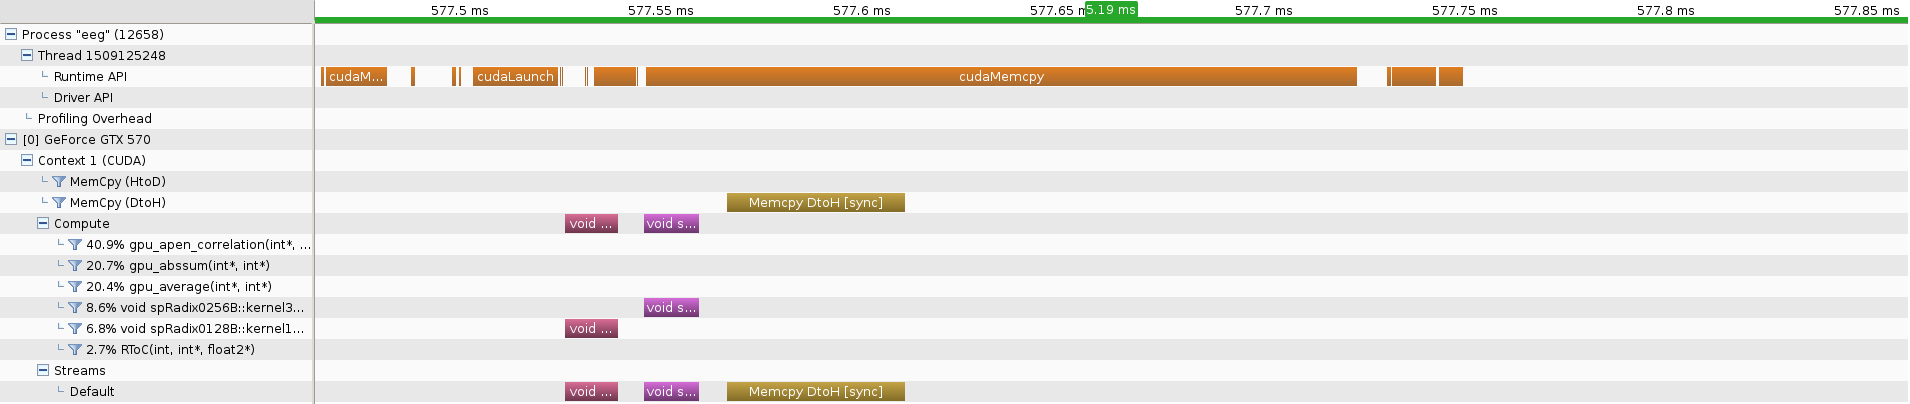
\includegraphics[scale=0.35]{images/10_cuda_fft_detail.PNG}
\caption{Detailed time-line of the execution of \texttt{cuFFT} for a single channel in NVVP. By far the most time is spent in the memory management functions.}
\label{fig:GPU_fft_detail}
\end{center}
\end{figure}

To port the C code to \texttt{CUDA}, the header and make file need to be edited. Also, documentation on converting data-types (e.g. real2complex: \texttt{RToC}, complex2complex: \texttt{CToC}) needs to be understood to optimize the algorithm. Some code is included below for reference:

\noindent Reference: Include the \texttt{cufft.h} at the top of the \texttt{fft.cu} file.
\begin{lstlisting}
#include "eeg.h"
#ifndef CPU_ONLY
	#include "cufft.h"
#endif
\end{lstlisting}

\noindent Reference: Edit \texttt{user flags} in the \texttt{make file}
\begin{lstlisting}
# Extra user flags
EXTRA_NVCCFLAGS ?=
EXTRA_LDFLAGS   ?= -lcufft
\end{lstlisting}

\noindent Reference: Add \texttt{RToC} the \texttt{fft.cu} file.
\begin{lstlisting}
__global__ 
void RToC(int size, int* input, float2* output)
{
	// Real to complex code from Greg Bryan
	int i = blockIdx.x * blockDim.x + threadIdx.x;

	if (i < size)
	{
		output[i].x = (float) input[i];
		output[i].y = 0;
	}
}
\end{lstlisting}

\noindent Reference: Perform \texttt{FFT} in \texttt{CUDA} using the \texttt{cufft.h} library functions.
\begin{lstlisting}
	float2 X[N];
	int* device_x;
	cudaMalloc((void**)&device_x, N*sizeof(int));
	cudaMemcpy(device_x , x, N*sizeof(int), cudaMemcpyHostToDevice);
	float2* device_xx;
	cudaMalloc((void**)&device_xx, N*sizeof(float2));
	int threads = 128;
	int block = N/threads;
	RToC<<<block, threads>>>(N, device_x, device_xx);
	cufftHandle plan;
	cufftPlan1d(&plan, N, CUFFT_C2C, 1);
	cufftExecC2C(plan, device_xx, device_xx, CUFFT_FORWARD);
	cudaMemcpy(X , device_xx, N*sizeof(float2), cudaMemcpyDeviceToHost);
	cufftDestroy(plan);
	cudaFree(device_xx);
\end{lstlisting}

\section{Optimization Results}

\begin{table}[h!]
\begin{center}  
\begin{tabular}{| l | c | c | c | c |}
\hline
\rowcolor[HTML]{c0c0c0}
\multicolumn{1}{| c |}{Feature} & \multicolumn{4}{c |}{Execution Time [s]} \\ \hline
Butterworth Filter & 0.000425 & 0.000425 & 0.000419 & 0.000516\\ \hline
Standard Features & 0.000528 & \cellcolor[HTML]{c0c0c0}0.001224 & \cellcolor[HTML]{c0c0c0}0.001061 & \cellcolor[HTML]{c0c0c0}0.001009\\ \hline
Peak to Peak Features & 0.000244 & 0.000275 & 0.000266 & 0.000322\\ \hline
Approximate Entropy Feature & 11.59626 & 11.59314 & \cellcolor[HTML]{c0c0c0}0.000903 & \cellcolor[HTML]{c0c0c0}0.000822\\ \hline
Hurst Coefficient Feature & 0.001433 & 0.001451 & 0.001409 & 0.001650\\ \hline
Power Spectral Density Feature & 0.019645 & 0.019494 & 0.019288 & \cellcolor[HTML]{c0c0c0} 0.001657\textbf{*}\\ \hline
\end{tabular}
\caption{Execution time of \texttt{EEG} application with incremental functionality ports to GPU. The darker background indicates that the specific feature was run on the GPU for that execution.\\
\textbf{*}The runtime for first channel of the \texttt{PSD} feature is $0.198508s$. The average runtime for the remaining $22$ channels is depicted in the table because the much higher runtime in for the first channel is a result of the time it takes to load the \texttt{cufft.h} library.}
\label{tab:GPU}
\end{center}
\end{table}

\begin{figure}[H]
\begin{center}
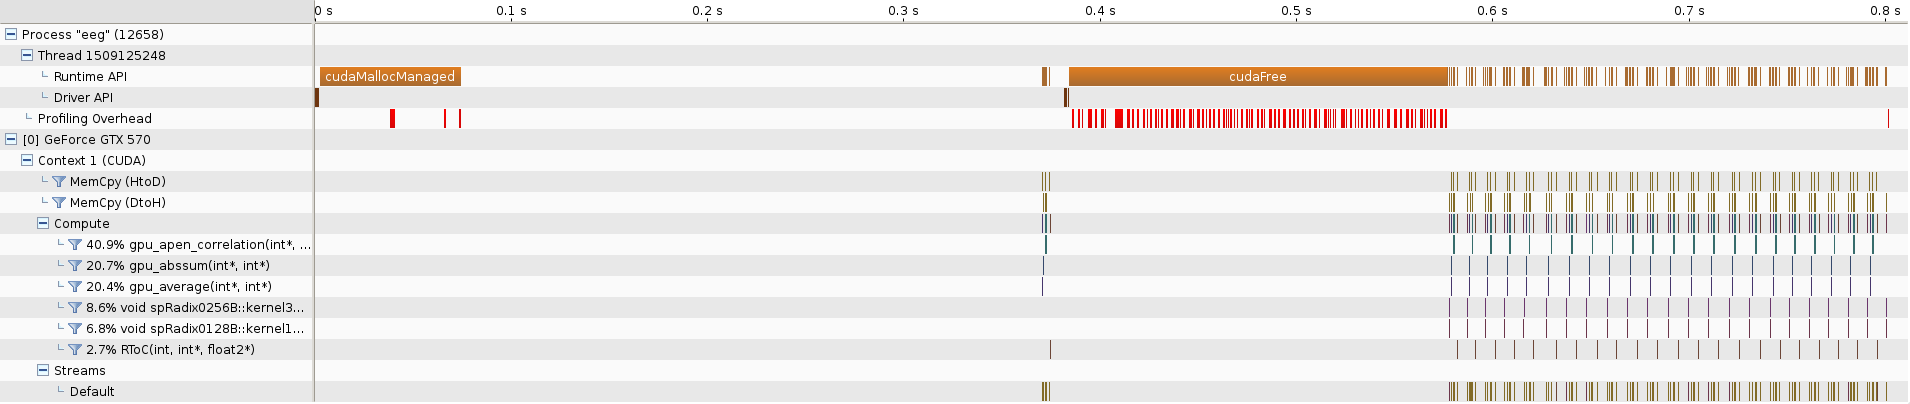
\includegraphics[scale=0.35]{images/08_cuda_all.PNG}
\caption{Execution time-line of the final version of the EEG application in NVVP. The warm-up period of about $0.6s$ can be seen in this figure, as well as the kernels that run the ported algorithms on the GPU.}
\label{fig:malloc}
\end{center}
\end{figure}

\section{Conclusion}

As can be seen from the optimization results, certain heavy-burdened features (\texttt{ApEn}, \texttt{PSD}) were improved with porting to the GPU. However, it is also noticed that features with negligible impacts (\texttt{abssum}) to the overall performance become more inefficient in small datasets. This is intuitive, since the GPU and CPU need to communicate with each other and the GPU requires a small warm-up period for each batch. 

Therefore, a GPU should only be used whenever the specific task is computationally heavy for the CPU, and the CPU could be better used to process other tasks. In general, the CPU is faster and takes less effort to use than incorporating a GPU, since specific functions/features need to be communicated effectively to the GPU.

To optimize the EEG application further, the nice modular structure it currently has needs to be compromised. If the algorithms of the features would be further intertwined, a significant amount of the time spent in the \texttt{cudaFree} and \texttt{cudaMallocManaged} functions can be reduced. This is a compromise that can bring a plethora of problems and should only be attempted with precaution because it makes the maintainability of the code much harder. However, in an ideal case you load the data into the GPU memory one, run all the features and then free the memory, in order to reduce the cost of the overhead as much as possible.

One other topic to address is the usage of multiple GPUs. If we had a much larger dataset the use of multiple GPUs would have a great impact on the execution time. On the GPUs on the test server this requires that the data is distributed correctly over the GPUs for each of the algorithms. Multiple GPU experiments are not reported since focusing on one GPU allows for a better comparison between the CPU and GPU architecture. However, similar considerations as above can be extrapolated, implying this architecture should only be used when there are large datasets or the CPU is running multiple tasks that could be better suited for GPUs.

\section{Notes}
Always \texttt{make clean} when changing the files that are being compiled (file name, included files, etc.), to avoid runtime errors, fragmentation errors and output mismatches.

\begin{thebibliography}{9}
\bibitem{User Guide}

Cookbook Tutorial:
\\
\url{https://devblogs.nvidia.com/easy-introduction-cuda-c-and-c/}
\\

Images from ECA course:
\\
\url{https://oncourse.tue.nl/2017/pluginfile.php/36505/mod_resource/content/1/ch9.pdf}
\\

John Nickolls, Ian Buck, Michael Garland, and Kevin Skadron. 2008. Scalable Parallel Programming with \texttt{CUDA}. Queue 6, 2 (March 2008), 40-53. DOI:
\\
\url{https://doi.org/10.1145/1365490.1365500}
\\    

cuFFT Library:
\\
\url{http://developer.download.nvidia.com/compute/cuda/1.0/CUFFT_Library_1.0.pdf}   
\\

CUDA profiler:
\\
\url{https://docs.nvidia.com/cuda/profiler-users-guide/index.html}   
\\

MobaXterm:
\\
\url{https://mobaxterm.mobatek.net/}


\end{thebibliography}

\section{Appendices}
\subsection{Test System Specifications}

\begin{figure}[H]
\begin{center}
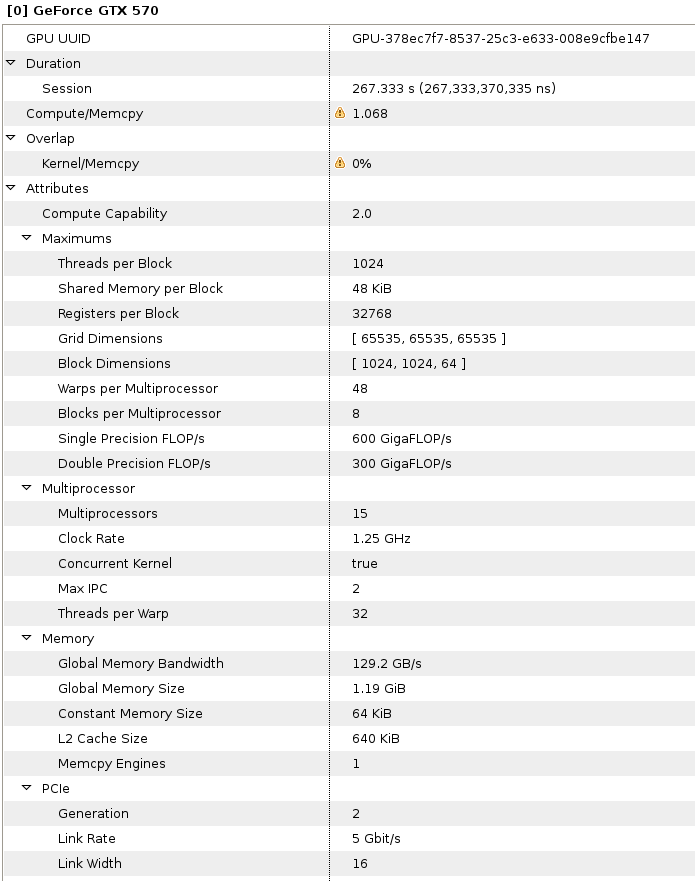
\includegraphics[scale=0.5]{images/GPU_properties.PNG}
\caption{Test System Parameters/Specifications}
\label{fig:gpu}
\end{center}
\end{figure}

\subsection{\texttt{CUDA Profiler}}
\begin{lstlisting}
~$ make profile
g++ -MMD -MF bw0_int.d -I/usr/local/cuda/include -I. -c -O3 -Wall bw0_int.c -o bw0_int.o
g++ -MMD -MF hurst.d -I/usr/local/cuda/include -I. -c -O3 -Wall hurst.c -o hurst.o
g++ -MMD -MF p2p.d -I/usr/local/cuda/include -I. -c -O3 -Wall p2p.c -o p2p.o
nvcc -m64  -Wno-deprecated-gpu-targets -gencode arch=compute_20,code=sm_20 -I/usr/local/cuda/include -I. -c apen.cu -o apen.o
nvcc -m64  -Wno-deprecated-gpu-targets -gencode arch=compute_20,code=sm_20 -I/usr/local/cuda/include -I. -c eeg.cu -o eeg.o
eeg.cu(73): warning: variable "read" was set but never used

eeg.cu(73): warning: variable "read" was set but never used

nvcc -m64  -Wno-deprecated-gpu-targets -gencode arch=compute_20,code=sm_20 -I/usr/local/cuda/include -I. -c fft.cu -o fft.o
nvcc -m64  -Wno-deprecated-gpu-targets -gencode arch=compute_20,code=sm_20 -I/usr/local/cuda/include -I. -c stafeature.cu -o stafeature.o
g++ bw0_int.o hurst.o p2p.o  apen.o eeg.o fft.o stafeature.o -L /usr/local/cuda/lib64 -lOpenCL -lcudart -lcufft -o eeg
nvprof --system-profiling on ./eeg
==23020== NVPROF is profiling process 23020, command: ./eeg
but,sta,p2p,ape,hur,pow;
0.000462,0.001623,0.000271,0.000946,0.001448,0.202044;
0.000426,0.000867,0.000267,0.000722,0.001453,0.002676;
0.000425,0.000878,0.000302,0.000766,0.001605,0.002705;
0.000562,0.001042,0.000368,0.000822,0.001958,0.002693;
0.000531,0.000961,0.000339,0.000778,0.001706,0.002912;
0.000511,0.000978,0.000325,0.000781,0.002053,0.002888;
0.000510,0.000958,0.000327,0.000778,0.001612,0.002694;
0.000424,0.000818,0.000263,0.000737,0.001367,0.002743;
0.000426,0.001245,0.000337,0.001051,0.001761,0.002803;
0.000485,0.000995,0.000358,0.000783,0.001676,0.002608;
0.000570,0.000975,0.000335,0.000790,0.001971,0.002653;
0.000536,0.000987,0.000318,0.000777,0.001674,0.002601;
0.000515,0.000939,0.000317,0.000775,0.001671,0.002950;
0.000508,0.000972,0.000349,0.000797,0.001796,0.003035;
0.000517,0.000938,0.000328,0.000773,0.001680,0.002879;
0.000519,0.001000,0.000325,0.000771,0.001690,0.003439;
0.000536,0.001228,0.000327,0.001060,0.001767,0.002791;
0.000541,0.000981,0.000307,0.000782,0.001676,0.002628;
0.000481,0.000939,0.000322,0.000783,0.001687,0.002608;
0.000502,0.000951,0.000320,0.000775,0.001694,0.002612;
0.000536,0.000968,0.000326,0.000791,0.001903,0.002958;
0.000520,0.000960,0.000315,0.000778,0.001671,0.002947;
0.000536,0.000966,0.000338,0.000812,0.001759,0.002941;

Feature 0: -0.120867
Feature 1: 37.755878
Feature 2: 648779.812500
Feature 3: 18188.429688
Feature 4: 73.820732
Feature 5: 95.777206
Feature 6: 0.017985
Feature 7: 0.518259
Feature 8: 38.066723
Feature 9: 46.835285
Feature 10: 75.471153
Feature 11: 439.958221
Feature 12: 745.191406
Feature 13: 1345.522827
Total time: 0.645091s
==23020== Profiling application: ./eeg
==23020== Profiling result:
Time(%)      Time     Calls       Avg       Min       Max  Name
 26.14%  1.7302ms        69  25.074us  24.767us  25.631us  [CUDA memcpy HtoD]
 21.65%  1.4331ms        46  31.153us  30.756us  31.538us  gpu_apen_correlation(int*, double*, int, unsigned int, double)
 20.64%  1.3661ms       115  11.879us  3.4230us  44.991us  [CUDA memcpy DtoH]
 10.99%  727.61us        23  31.635us  31.460us  32.041us  gpu_abssum(int*, int*)
 10.82%  715.90us        23  31.126us  30.786us  33.339us  gpu_average(int*, int*)
  4.71%  311.82us        23  13.557us  13.308us  13.893us  void spRadix0256B::kernel3Mem<unsigned int, float, fftDirection_t=-1, unsigned int=16, unsigned int=2, L1, ALL, WRITEBACK>(kernel_parameters_t<fft_mem_radix3_t, unsigned int, float>)
  3.64%  240.68us        23  10.464us  9.3840us  13.460us  void spRadix0128B::kernel1Mem<unsigned int, float, fftDirection_t=-1, unsigned int=16, unsigned int=4, L1, ALL, WRITEBACK>(kernel_parameters_t<fft_mem_radix1_t, unsigned int, float>)
  1.41%  93.040us        23  4.0450us  3.4720us  4.9770us  RToC(int, int*, float2*)

==23020== System profiling result:
Device "GeForce GTX 570 (0)"
                         Count         Avg         Min         Max
     Temperature (C)        16       40.38       39.00       41.00
             Fan (%)         8       85.00       85.00       85.00
Device "GeForce GTX 570 (1)"
                         Count         Avg         Min         Max
     Temperature (C)        16       35.75       35.00       36.00
             Fan (%)         8       85.00       85.00       85.00
Device "GeForce GTX 570 (2)"
                         Count         Avg         Min         Max
     Temperature (C)        16       34.94       34.00       35.00
             Fan (%)         8       85.00       85.00       85.00

==23020== API calls:
Time(%)      Time     Calls       Avg       Min       Max  Name
 63.30%  205.59ms       208  988.39us     721ns  193.54ms  cudaFree
 21.62%  70.222ms         1  70.222ms  70.222ms  70.222ms  cudaMallocManaged
  4.86%  15.777ms       207  76.214us  6.5890us  214.76us  cudaMalloc
  4.50%  14.623ms        23  635.77us  567.78us  724.22us  cudaGetDeviceProperties
  3.20%  10.387ms       184  56.448us  19.569us  185.28us  cudaMemcpy
  1.24%  4.0393ms       498  8.1110us     187ns  327.77us  cuDeviceGetAttribute
  0.70%  2.2758ms       161  14.135us  6.9840us  44.682us  cudaLaunch
  0.17%  536.44us         6  89.406us  85.532us  94.035us  cuDeviceTotalMem
  0.15%  500.69us       736     680ns     406ns  25.071us  cudaFuncSetCacheConfig
  0.13%  415.74us         6  69.290us  61.466us  82.001us  cuDeviceGetName
  0.06%  186.02us       161  1.1550us     342ns  3.7340us  cudaGetDevice
  0.04%  114.00us       437     260ns     138ns  2.5830us  cudaSetupArgument
  0.03%  95.005us       161     590ns     252ns  7.3410us  cudaConfigureCall
  0.01%  17.399us        46     378ns     179ns     888ns  cudaPeekAtLastError
  0.00%  13.760us        46     299ns     209ns     352ns  cudaGetLastError
  0.00%  8.8440us         3  2.9480us  1.9550us  3.6090us  cuDeviceGetPCIBusId
  0.00%  4.6190us         9     513ns     240ns  1.2330us  cuDeviceGet
  0.00%  1.9140us         3     638ns     373ns     777ns  cuDeviceGetCount
  0.00%  1.3690us         1  1.3690us  1.3690us  1.3690us  cuInit
  0.00%  1.0910us         1  1.0910us  1.0910us  1.0910us  cuDriverGetVersion
\end{lstlisting}

\begin{comment}

NOTE: Cuda code for apen
\begin{lstlisting}
	#ifdef CPU_ONLY
	A = log(apen_correlation(np, x, m, r) / apen_correlation(np, x, m + 1, r));

	#else
	// GPU CODE
	dim3 dimBlock(BLOCK_SIZE,BLOCK_SIZE);
	dim3 dimGrid(GRID_SIZE,GRID_SIZE);
	cudaError_t err;
	int32_t* device_x;
	err=cudaMalloc(&device_x, np*sizeof(int32_t));
	cudaCheckError(err);
	double* device_blocksums;
	err=cudaMalloc(&device_blocksums, GRID_SIZE*GRID_SIZE*sizeof(double));  
	cudaCheckError(err);
	err=cudaMemcpy(device_x, x, np*sizeof(int32_t), cudaMemcpyHostToDevice);
	cudaCheckError(err);
	gpu_apen_correlation<<<dimGrid, dimBlock>>>(device_x, device_blocksums, np, m, r);
	//cudaCheckError(cudaPeekAtLastError()); 
	double blocksums[GRID_SIZE*GRID_SIZE];
	err=cudaMemcpy(blocksums, device_blocksums, GRID_SIZE*GRID_SIZE*sizeof(double), cudaMemcpyDeviceToHost); 
	cudaCheckError(err);
	err=cudaFree(device_blocksums);
	cudaCheckError(err);
	int idxi;
	double sum = 0;
	for(idxi=0;idxi<GRID_SIZE*GRID_SIZE;idxi++){
		sum += ((double) blocksums[idxi]); 
	}
	err=cudaMalloc(&device_blocksums, GRID_SIZE*GRID_SIZE*sizeof(double));  
	cudaCheckError(err); 
	gpu_apen_correlation<<<dimGrid, dimBlock>>>(device_x, device_blocksums, np, m + 1, r);
	//cudaCheckError(cudaPeekAtLastError()); 
	err=cudaMemcpy(blocksums, device_blocksums, GRID_SIZE*GRID_SIZE*sizeof(double), cudaMemcpyDeviceToHost); 
	cudaCheckError(err);
	err=cudaFree(device_x);
	cudaCheckError(err);
	err=cudaFree(device_blocksums);
	cudaCheckError(err);
	double sum2 = 0;
	for(idxi=0;idxi<GRID_SIZE*GRID_SIZE;idxi++){
		sum2 += ((double) blocksums[idxi]); 
	}
	A = log(sum / sum2);
	#endif
\end{lstlisting}

\end{comment}

\end{document}
